\documentclass[11pt,a4paper]{article}
\usepackage[spanish]{babel}					% Utilizar español
\usepackage[utf8]{inputenc}					% Caracteres UTF-8
\usepackage{graphicx}						% Imagenes
\usepackage[hidelinks]{hyperref}			% Poner enlaces sin marcarlos en rojo
\usepackage{fancyhdr}						% Modificar encabezados y pies de pagina
\usepackage{float}							% Insertar figuras
\usepackage[textwidth=390pt]{geometry}		% Anchura de la pagina
\usepackage[nottoc]{tocbibind}				% Referencias (no incluir num pagina indice en Indice)
\usepackage{sectsty}						% Secciones sin enumeración
\usepackage{enumitem}						% Enumeraciones
\usepackage{mathtools}
\usepackage{amsmath}
\usepackage{amssymb}

\newcommand{\sign}{\text{sign}}

% Configuracion de encabezados y pies de pagina
\pagestyle{fancy}
\lhead{Vladislav Nikolov Vasilev}
\rhead{Aprendizaje Automático}
\lfoot{Grado en Ingeniería Informática}
\cfoot{}
\rfoot{\thepage}
\renewcommand{\headrulewidth}{0.4pt}		% Linea cabeza de pagina
\renewcommand{\footrulewidth}{0.4pt}		% Linea pie de pagina

\begin{document}
\pagenumbering{gobble}

% Pagina de titulo
\begin{titlepage}

\begin{minipage}{\textwidth}

\centering


\includegraphics[scale=0.5]{img/ugr.png}\\

\textsc{\Large Aprendizaje Automático\\[0.2cm]}
\textsc{GRADO EN INGENIERÍA INFORMÁTICA}\\[1cm]

\noindent\rule[-1ex]{\textwidth}{1pt}\\[1.5ex]
\textsc{{\Huge MEMORIA PRÁCTICA 1\\}}
\noindent\rule[-1ex]{\textwidth}{2pt}\\[3.5ex]

\end{minipage}

\vspace{1.5cm}

\begin{minipage}{\textwidth}

\centering

\textbf{Autor}\\ {Vladislav Nikolov Vasilev}\\[2.5ex]
\textbf{Rama}\\ {Computación y Sistemas Inteligentes}\\[2.5ex]
\vspace{0.3cm}


\includegraphics[scale=0.3]{img/etsiit.jpeg}

\vspace{0.7cm}
\textsc{Escuela Técnica Superior de Ingenierías Informática y de Telecomunicación}\\
\vspace{1cm}
\textsc{Curso 2018-2019}
\end{minipage}
\end{titlepage}

\pagenumbering{arabic}
\tableofcontents
\thispagestyle{empty}				% No usar estilo en la pagina de indice

\newpage

\section{Ejercicio sobre la búsqueda iterativa de óptimos}

\subsection*{Apartado 1}
\noindent Implementar el algoritmo de gradiente descendente.\\

A continuación se muestra el código en Python implementado:

\begin{figure}[H]
\centering
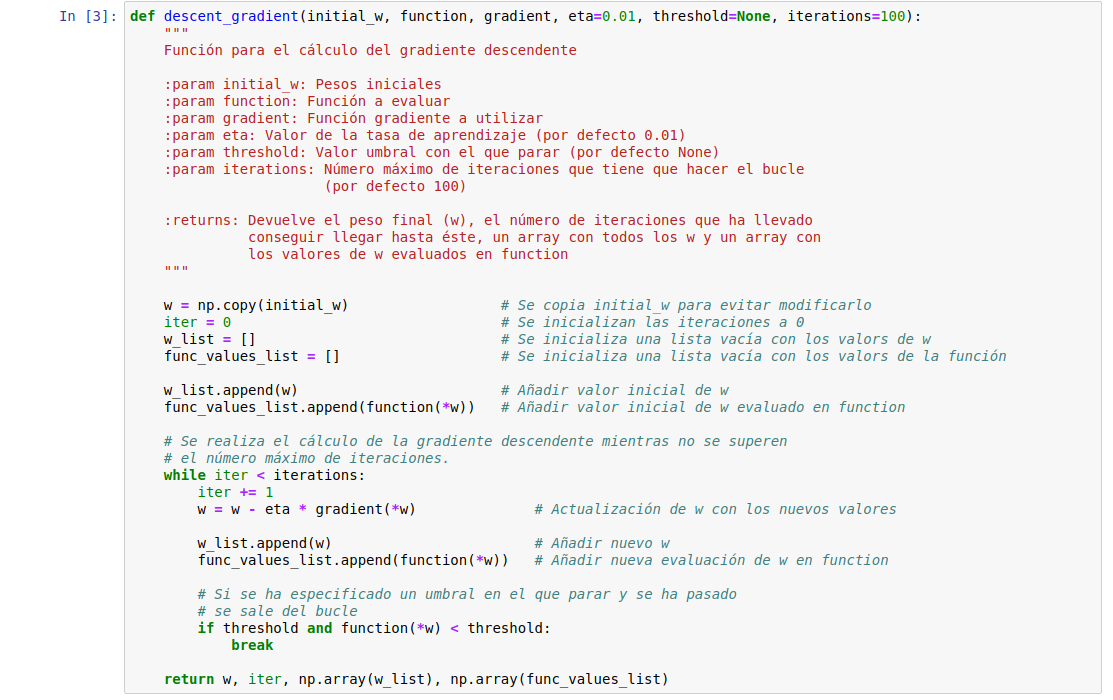
\includegraphics[scale=0.4]{img/descent_gradient_implementation.png}
\end{figure}


Se ha intentado que esta implementación sea lo más general posible para poder utilizarla en los ejercicios
posteriores, parametrizando la función que recibe (parámetro \textbf{function}), la cuál puede ser tanto
$f(x, y)$ como $E(u, v)$. Con este motivo, también se ha parametrizado el error con el que se quiere ajustar,
ya que en un caso no será necesario utilizar un error como criterio de parada (de ahí que su valor por defecto
sea \textbf{None}). Y, adicionalmente, se ha parametrizado el gradiente (parámetro \textbf{gradient}), para que
también se pueda especificar a la hora de la llamada cuál se usará. \\

\subsection*{Apartado 2}
\noindent Considerar la función $E(u, v) = (u^2 e^v - 2 v^2 e^{-u})^2$. Usar gradiente descendente para encontrar un
mínimo de esta funcón, comenzando desde el punto $(u, v) = (1, 1)$ y usanto una tasa de aprendizaje $\eta = 0.01$.

\begin{enumerate}[label=\alph*)]
	\item Calcular analíticamente y mostrar la expresión del gradiente de la función $E(u, v)$.
\end{enumerate}

Para calcular el gradiente, vamos a calcular antes $\frac{\partial E}{\partial u}$ y $\frac{\partial E}{\partial v}$.
Las derivadas, al aplicar la regla de la cadena, quedarían de la siguiente forma:

\begin{equation}
\begin{split}
\frac{\partial E}{\partial u}&= \frac{\partial}{\partial u} \Big( (u^2 e^v - 2 v^2 e^{-u})^2 \Big) = 2(u^2 e^v - 2 v^2 e^{-u})
\frac{\partial (u^2 e^v - 2 v^2 e^{-u})}{\partial u} = \\
 &=  2(u^2 e^v - 2 v^2 e^{-u})(2ue^v + 2 v^2 e^{-u})
\end{split}
\end{equation}

\begin{equation}
\begin{split}
\frac{\partial E}{\partial v}&= \frac{\partial}{\partial v} \Big( (u^2 e^v - 2 v^2 e^{-u})^2 \Big) = 2(u^2 e^v - 2 v^2 e^{-u})
\frac{\partial (u^2 e^v - 2 v^2 e^{-u})}{\partial v} = \\
 &=  2(u^2 e^v - 2 v^2 e^{-u})(u^2 e^v -4 v e^{-u})
\end{split}
\end{equation}

Con esto, tenemos que la expresión del gradiente es la siguiente:

\begin{equation}
\nabla E =
\left[
{
\begin{array}{c}
	\frac{\partial E}{\partial u} \\
	\\
	\frac{\partial E}{\partial v}
\end{array}
}
\right]
\end{equation}

\begin{equation}
\nabla E =
\left[
{
\begin{array}{c}
	2(u^2 e^v - 2 v^2 e^{-u})(2ue^v + 2 v^2 e^{-u}) \\
	\\
	2(u^2 e^v - 2 v^2 e^{-u})(u^2 e^v -4 v e^{-u})
\end{array}
}
\right]
\end{equation}

\begin{enumerate}[resume, label=\alph*)]
	\item ¿Cuántas iteraciones tarda el algoritmo en obtener por primera vez un valor de $E(u, v)$ inferior a $10^{-14}$?
	(Usar flotantes de 64 bits)
\end{enumerate}

\begin{figure}[H]
\centering
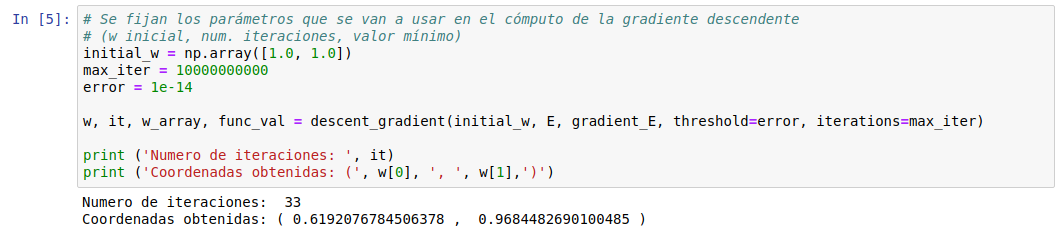
\includegraphics[scale=0.4]{img/jnbook_ej_2.png}
\caption{Cálculo del mínimo mediante el Gradiente Descendente para la función $E(u, v)$.}
\end{figure}

Como se puede ver en la figura anterior, donde también se incluye el código, el algoritmo tarda 33 iteraciones en encontrar
por primera vez un valor de $E(u, v)$ inferior a $10^{-14}$.

\begin{enumerate}[resume, label=\alph*)]
	\item ¿En qué coordenadas $(u, v)$ se alcanzó por primera vez un valor igual o menor a $10^{-14}$ en el apartado anterior?
\end{enumerate}

Las coordenadas donde se alcanzó un valor inferior a $10^{-14}$ son $(0.619, 0.968)$ (redondeadas a 3 cifras decimales).

\subsection*{Apartado 3}
\noindent Considerar ahora la función $f(x, y) = x^2 + 2y^2 + 2\sin(2 \pi x)\sin(2 \pi y)$.

\begin{enumerate}[label=\alph*)]
	\item Usar gradiente descendente para minimizar esta función. Usar como punto inicial $(x_0 = 0.1, y_0 = 0.1)$,
	tasa de aprendizaje $\eta = 0.01$ y un máximo de 50 iteraciones. Repetir el experimento pero usando $\eta = 0.1$,
	comentar las diferencias y su dependencia de $\eta$.
\end{enumerate}

Antes de mostrar las gráficas, vamos a calcular el gradiente de la función $f(x, y)$. Primero, vamos a calcular 
$\frac{\partial f}{\partial x}$ y $\frac{\partial f}{\partial y}$:

\begin{equation}
\frac{\partial f}{\partial x} = \frac{\partial}{\partial x} \Big(x^2 + 2y^2 + 2\sin(2 \pi x)\sin(2 \pi y)\Big) =
2x + 4 \pi \cos(2 \pi x)\sin(2 \pi y)
\end{equation}

\begin{equation}
\frac{\partial f}{\partial y} = \frac{\partial}{\partial y} \Big(x^2 + 2y^2 + 2\sin(2 \pi x)\sin(2 \pi y)\Big) =
4y + 4 \pi \sin(2 \pi x)\cos(2 \pi  y)
\end{equation}

\begin{equation}
\nabla f =
\left[
{
\begin{array}{c}
	\frac{\partial f}{\partial x} \\
	\\
	\frac{\partial f}{\partial y}
\end{array}
}
\right]
\end{equation}

\begin{equation}
\nabla f =
\left[
{
\begin{array}{c}
	2x + 4 \pi \cos(2 \pi x)\sin(2 \pi y) \\
	\\
	4y + 4 \pi \sin(2 \pi x)\cos(2 \pi  y)
\end{array}
}
\right]
\end{equation} \\

Una vez calculada la expresión del gradiente, vamos a ejecutar el código y a realizar la comparación de los cálculos 
del gradiente al cambiar el valor de $\eta$:

\begin{figure}[H]
\centering
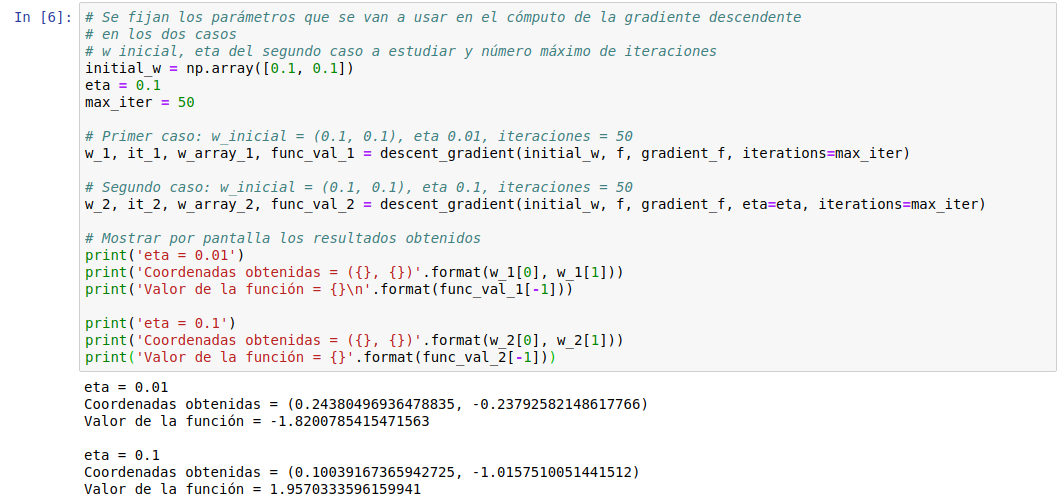
\includegraphics[scale=0.4]{img/jnbook_ej_3_a.png}
\caption{Valores de los óptimos para la función $f(x, y)$ cambiando $\eta$-}
\end{figure}

A continuación, se muestra el gráfico comparativo:

\begin{figure}[H]
\centering
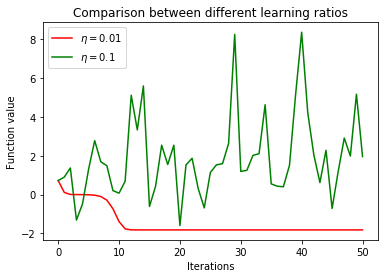
\includegraphics[scale=0.8]{img/comparison_lr.png}
\caption{Comparativa gráfica de la Gradiente Descendente con diferentes valores de $\eta$.}
\end{figure}

Como se puede ver, después de 50 iteraciones, al utilizar un $\eta = 0.01$ se consigue converger a un óptimo local, mientras
que al utilizar un $\eta = 0.1$ no se consigue. En el primer caso, los valores de $w$ van modificándose poco a poco con cada
iteración, y por eso en el gráfico que puede ver que tiene una forma muy suavizada el cambio que sufre $w$ entre iteración e
iteración. En cambio, en el segundo caso, al tener un $\eta$ mayor, se le da mucho peso al gradiente, y por tanto, los
valores de $w$ van modificándose muy bruscamente, como si estuviese oscilando entre la parte previa al mínimo y la
posterior, sin llegar a converger en ningún momento.\\

Por tanto, el valor de $\eta$ juega un factor clave en el algoritmo del descenso de gradiente. Si es muy bajo, los valores
de $w$ van descendiendo poco a poco, pero si el número de iteraciones son suficientes, se asegura llegar a un óptimo local.
Sin embargo, si el $\eta$ es muy grande, no se asegura en ningún momento que se pueda llegar al óptimo local, ya que puede
ir saltando entre la parte anterior y la posterior al mínimo indefinidamente, llegando incluso a poder alejarse de éste.

\begin{enumerate}[resume, label=\alph*)]
	\item Obtener el valor mínimo y los valores de las variables $(x, y)$ en donde se alcanzan cuando el punto de inicio
	se fija: $(0.1, 0.1), (1, 1), (-0.5, -0.5), (-1, -1)$. Generar una tabla con los valores obtenidos.
\end{enumerate}

A continuación se muestra una captura de pantalla con el código que permite generar los datos y la salida en formato tabla,
donde se muestran los 4 puntos con sus coordenadas iniciales, finales y valor del punto final.

\begin{figure}[H]
\centering
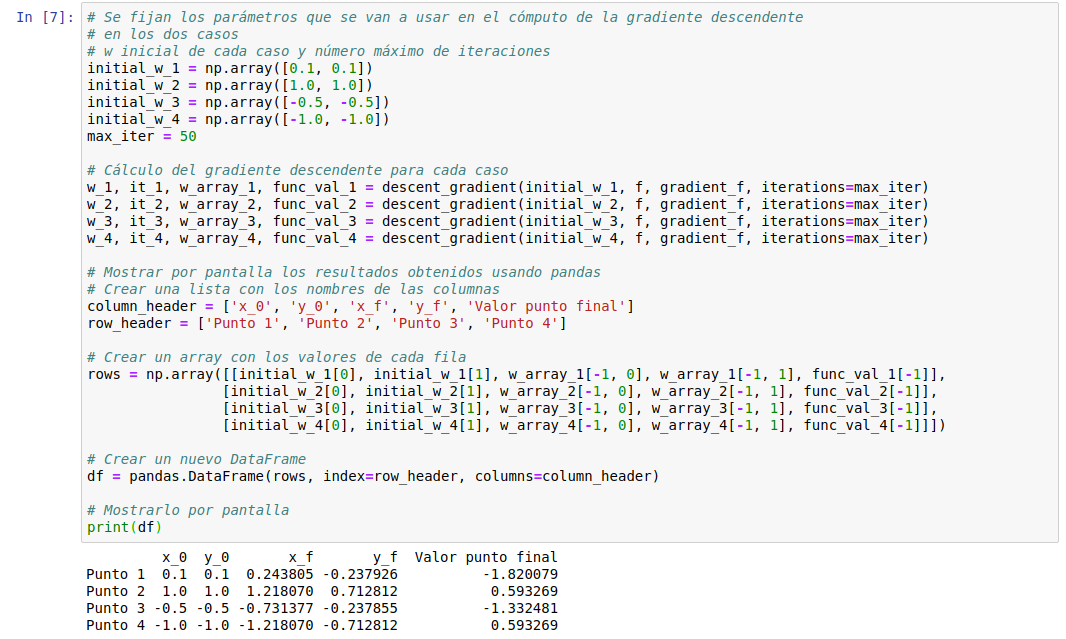
\includegraphics[scale=0.4]{img/jbook_ej_3_b.png}
\end{figure}

\subsection*{Apartado 4}
\noindent ¿Cuál sería su conclusión sobre la verdadera dificultad de encontrar el máximo global de una función arbitraria?\\

Encontrar el máximo global de una función arbitraria puede llegar a ser difícil y depende de una serie factores:

\begin{itemize}[label=\textbullet]
	\item \textbf{Forma de la función}: Si la función es convexa, como solo tiene un mínimo, es fácil encontrarlo con
	algoritmos como por ejemplo el Gradiente Descendente. Si la función tiene muchos óptimos locales o muchas curvaturas
	puede llegar a ser difícil dar con el óptimo global, y los algoritmos iterativos pueden llegar a quedarse en óptimos
	locales.
	\item \textbf{Punto de inicio}: El punto desde el que se empieza puede influir en el óptimo al que se llegue. En algunos
	casos, el punto inicial puede hacer que al aplicar algoritmos se llegue a un óptimo local y no se consiga salir de ahí.
	En otros casos, el punto puede estar más cerca del óptimo global, y por tanto se puede llegar a éste más fácilmente. Por
	tanto, hay que elegir con cuidado en qué punto se debería empezar.
	\item \textbf{El ratio de aprendizaje $(\eta)$}: En algunos algoritmos, como por ejemplo el Gradiente Descendente y sus
	variantes, se utiliza un ratio de aprendizaje que permite dar más o menos peso al gradiente a la hora de acutalizar los
	valores de $w$. En caso de escoger un valor muy pequeño, la velocidad a la que se va a converger a un óptimo será más
	lenta, y por tanto se necesitarán más iteraciones. Un ratio muy elevado hará que sea muy difícil converger, ya que el
	valor de $w$ irá pegando muchos saltos. Por tanto, un ratio de aprendizaje adecuado hará que se pueda llegar a un óptimo
	de mejor o peor forma. Dicho esto, ninguno de los dos garantiza que el óptimo al que se acabe llegando sea global, ya
	que perfectamente puede llegar a un óptimo local y quedarse ahí.
\end{itemize}

\section{Ejercicio sobre Regresión Lineal}

Este ejercicio ajusta modelos de regresión a vectores de características extraidos de imágenes de digitos manuscritos. En
particular se extraen dos característcas concretas: el valor medio del nivel de gris y simetría del número respecto de su eje
vertical. Solo se seleccionarán para este ejercicio las imágenes de los números 1 y 5.

\subsection*{Apartado 1}
Estimar un modelo de regresión lineal a partir de los datos proporcionados de dichos números (Intensidad promedio, Simetria)
usando tanto el algoritmo de la pseudoinversa como Gradiente descendente estocástico (SGD). Las etiquetas serán
$ \lbrace -1, 1 \rbrace $, una para cada vector de cada uno de los números. Pintar las soluciones obtenidas junto con los
datos usados en el ajuste. Valorar la bondad del resultado usando $E_{in}$ y $E_{out}$ (para $E_{out}$ calcular las
predicciones usando los datos del fichero de test). ( usar $Regress\_Lin(datos, label)$ como llamada para la función
(opcional)).\\

Primero, vamos a observar las funciones implementadas para realizar los ajustes:

\begin{figure}[H]
\centering
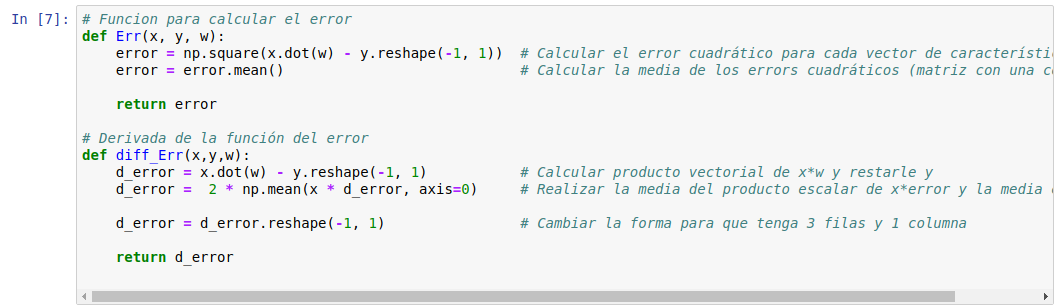
\includegraphics[scale=0.4]{img/func_error.png}
\caption{Función de error y derivada de ésta para el gradiente.}
\end{figure}

\begin{figure}[H]
\centering
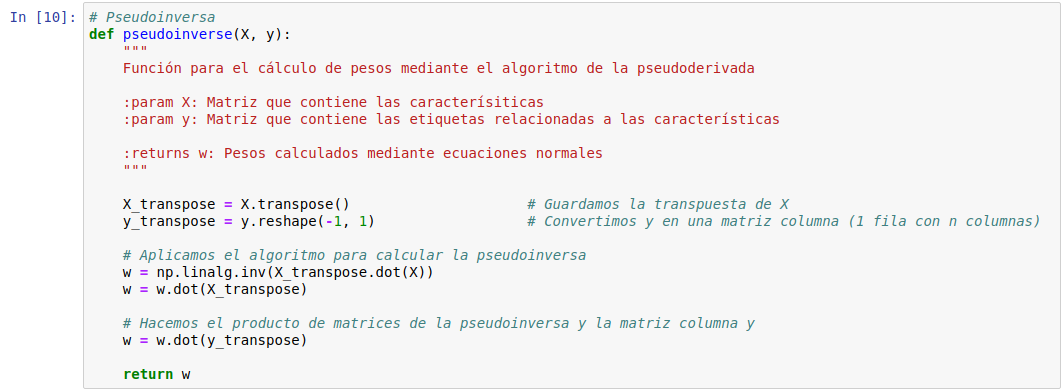
\includegraphics[scale=0.4]{img/pseudoinverse.png}
\caption{Implementación del algoritmo de la pseudoinversa.}
\end{figure}

\begin{figure}[H]
\centering
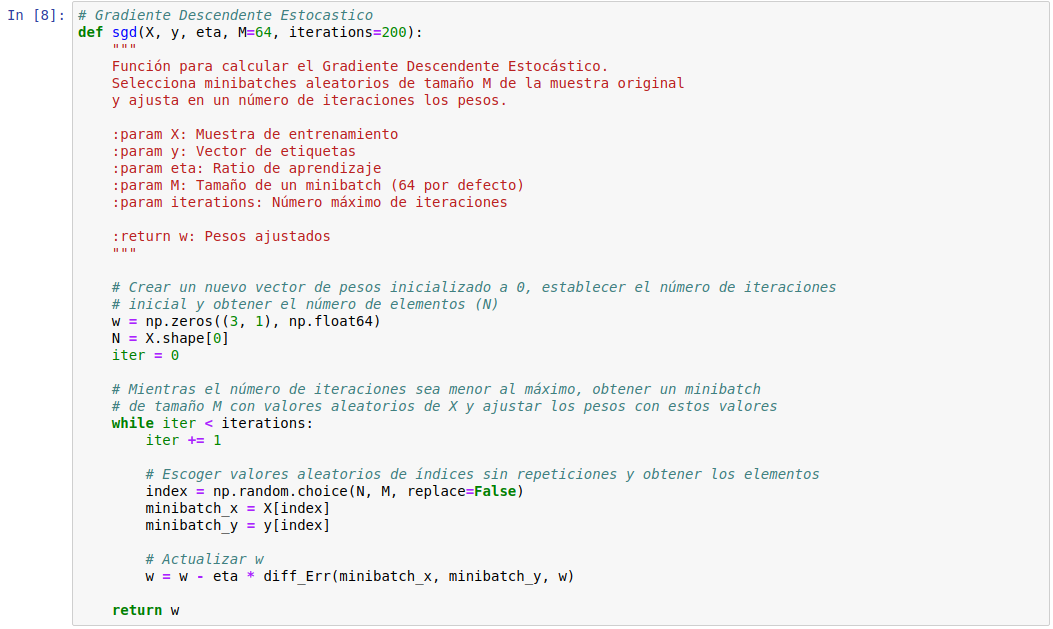
\includegraphics[scale=0.4]{img/sgd.png}
\caption{Implementación del Gradiente Descendente Estocástico.}
\end{figure}


\subsection*{Apartado 2}
\noindent En este apartado exploramos como se transforman los errores $E_{in}$ y $E_{out}$ cuando aumentamos la complejidad
del modelo lineal usado. Ahora hacemos uso de la función $simula\_unif (N, 2, size)$ que nos devuelve $N$ coordenadas 2D de
puntos uniformemente muestreados dentro del cuadrado definido por $[-size, size] \times [-size, size]$

\begin{itemize}
	\item EXPERIMENTO
	\begin{enumerate}[label=\alph*)]
		\item Generar una muestra de entrenamiento de $N = 1000$ puntos en el cuadrado $X = [-1, 1] \times [-1, 1]$.
		Pintar el mapa de puntos 2D. (ver función de ayuda)
	\end{enumerate}
	
	\begin{enumerate}[resume, label=\alph*)]
		\item Consideremos la función $f(x_1, x_2) = \sign((x_1 - 0.2)^2 + x_2^2 - 0.6)$ que usaremos para asignar una
		etiqueta a cada punto de la muestra anterior. Introducimos ruido sobre las etiquetas cambiando aleatoriamente
		el signo de un 10\% de las mismas. Pintar el mapa de etiquetas obtenido.
	\end{enumerate}
	
	\begin{enumerate}[resume, label=\alph*)]
		\item Usando como vector de características $(1, x_1, x_2)$ ajustar un modelo de regresión lineal al conjunto de
		datos generado y estimar los pesos $w$. Estimar el error de ajuste $E_{in}$ usando Gradiente Descendente Estocástico
		(SGD).
	\end{enumerate}
	
	\begin{enumerate}[resume, label=\alph*)]
		\item Ejecutar todo el experimento definido por (a)-(c) 1000 veces (generamos 1000 muestras diferentes) y
		\begin{itemize}
			\item Calcular el valor medio de los errores $E_{in}$ de las 1000 muestras.
			\item Generar 1000 puntos nuevos por cada iteración y calcular con ellos el valor de $E_{out}$ en dicha iteración.
			Calcular el valor medio de $E_{out}$ en todas las iteraciones.
		\end{itemize}
	\end{enumerate}
	
	\begin{enumerate}[resume, label=\alph*)]
		\item Valore que tan bueno considera que es el ajuste con este modelo lineal a la vista de los valores medios
		obtenidos de $E_{in}$ y $E_{out}$.
	\end{enumerate}
\end{itemize}


\section{Bonus}

\subsection*{Apartado 1}
\noindent \textbf{Método de Newton}. Implementar el algoritmo de minimización de Newton y aplicarlo a la función $f(x, y)$
dada en el ejercicio 3. Desarrolle los mismos experimentos usando los mismos puntos de inicio.

\begin{itemize}
	\item Generar un gráfico de como desciende el valor de la función con las iteraciones.
	\item Extraer conclusiones sobre las conductas de los algoritmos comparando la curva de decrecimiento de la función
	calculada en el apartado anterior y la correspondiente obtenida con el gradiente descendente.
\end{itemize}

\newpage

\begin{thebibliography}{5}

\bibitem{nombre-referencia}
Texto referencia
\\\url{https://url.referencia.com}

\end{thebibliography}

\end{document}

